\documentclass{article}

\usepackage{fancyhdr}
\usepackage{extramarks}
\usepackage{amsmath}
\usepackage{amsthm}
\usepackage{amsfonts}
\usepackage{tikz}
\usepackage[plain]{algorithm}
\usepackage{algpseudocode}

\usetikzlibrary{automata,positioning}

%
% Basic Document Settings
%

\topmargin=-0.45in
\evensidemargin=0in
\oddsidemargin=0in
\textwidth=6.5in
\textheight=9.0in
\headsep=0.25in

\linespread{1.1}

\pagestyle{fancy}
\lhead{\hmwkAuthorName}
\chead{\hmwkClass\ (\hmwkClassInstructor\ \hmwkClassTime): \hmwkTitle}
\rhead{\firstxmark}
\lfoot{\lastxmark}
\cfoot{\thepage}

\renewcommand\headrulewidth{0.4pt}
\renewcommand\footrulewidth{0.4pt}

\setlength\parindent{0pt}

%
% Create Problem Sections
%

\newcommand{\enterProblemHeader}[1]{
    \nobreak\extramarks{}{Question \arabic{#1} continued on next page\ldots}\nobreak{}
    \nobreak\extramarks{Question \arabic{#1} (continued)}{Question \arabic{#1} continued on next page\ldots}\nobreak{}
}

\newcommand{\exitProblemHeader}[1]{
    \nobreak\extramarks{Question \arabic{#1} (continued)}{Question \arabic{#1} continued on next page\ldots}\nobreak{}
    \stepcounter{#1}
    \nobreak\extramarks{Question \arabic{#1}}{}\nobreak{}
}

\setcounter{secnumdepth}{0}
\newcounter{partCounter}
\newcounter{homeworkProblemCounter}
\setcounter{homeworkProblemCounter}{1}
\nobreak\extramarks{Question \arabic{homeworkProblemCounter}}{}\nobreak{}

%
% Homework Problem Environment
%
% This environment takes an optional argument. When given, it will adjust the
% problem counter. This is useful for when the problems given for your
% assignment aren't sequential. See the last 3 problems of this template for an
% example.
%
\newenvironment{homeworkProblem}[1][-1]{
    \ifnum#1>0
        \setcounter{homeworkProblemCounter}{#1}
    \fi
    \section{Question \arabic{homeworkProblemCounter}}
    \setcounter{partCounter}{1}
    \enterProblemHeader{homeworkProblemCounter}
}{
    \exitProblemHeader{homeworkProblemCounter}
}

%
% Homework Details
%   - Title
%   - Due date
%   - Class
%   - Section/Time
%   - Instructor
%   - Author
%

\newcommand{\hmwkTitle}{Assignment\ \#1}
\newcommand{\hmwkDueDate}{February 27, 2018}
\newcommand{\hmwkClass}{AIC}
\newcommand{\hmwkClassTime}{}
\newcommand{\hmwkClassInstructor}{Dr. D. Seshachalam}
\newcommand{\hmwkAuthorName}{\textbf{A13}}

%
% Title Page
%

% \title{
%     \vspace{2in}
%     \textmd{\textbf{\hmwkClass:\ \hmwkTitle}}\\
%     \normalsize\vspace{0.1in}\small{Due\ on\ \hmwkDueDate\ at 3:10pm}\\
%     \vspace{0.1in}\large{\textit{\hmwkClassInstructor\ \hmwkClassTime}}
%     \vspace{3in}
% }

% \author{\hmwkAuthorName}
% \date{}

\renewcommand{\part}[1]{\textbf{\large Part \Alph{partCounter}}\stepcounter{partCounter}\\}

%
% Various Helper Commands
%

% Useful for algorithms
\newcommand{\alg}[1]{\textsc{\bfseries \footnotesize #1}}

% For derivatives
\newcommand{\deriv}[1]{\frac{\mathrm{d}}{\mathrm{d}x} (#1)}

% For partial derivatives
\newcommand{\pderiv}[2]{\frac{\partial}{\partial #1} (#2)}

% Integral dx
\newcommand{\dx}{\mathrm{d}x}

% Alias for the Solution section header
\newcommand{\solution}{\textbf{\large Solution}}

% Probability commands: Expectation, Variance, Covariance, Bias
\newcommand{\E}{\mathrm{E}}
\newcommand{\Var}{\mathrm{Var}}
\newcommand{\Cov}{\mathrm{Cov}}
\newcommand{\Bias}{\mathrm{Bias}}

\begin{document}

\title{\fontsize{14pt}{16.8pt}\selectfont\bf{ANALOG INTEGRATED CIRCUITS [15ES4GCAIC]}}
\date{}

\maketitle
\thispagestyle{empty}

\begin{center}
\vspace*{-15mm}

{\fontsize{14pt}{16.8pt}\selectfont\textbf{SELF STUDY}} \\
\vspace*{4mm}

{\fontsize{14pt}{16.8pt}\selectfont\textit{in}} \\
\vspace*{3mm}

{\fontsize{14pt}{16.8pt}\selectfont\textbf{ELECTRONICS AND COMMUNICATION ENGINEERING}} \\

\vspace*{4mm}
{\fontsize{14pt}{16.8pt}\selectfont\textit{by}} \\
\vspace*{5mm}

\author{\fontsize{14pt}{16.8pt}\selectfont\textbf{A. Vipula}}  \hspace*{12mm} {\fontsize{14pt}{16.8pt}\selectfont\textbf{Akshit Bhalla}} \hspace*{12mm} {\fontsize{14pt}{16.8pt}\selectfont\textbf{Amrutha M.}}\\
\vspace*{2mm}
{\fontsize{12pt}{14.4pt}\selectfont\textit{[1BM16EC007]} \hspace*{12mm} \selectfont\textit{[1BM16EC015]} \hspace*{12mm} \selectfont\textit{[1BM16EC018]} } \\



\vspace*{3mm}

\vspace*{4mm}\fontsize{14pt}{16.8pt}\selectfont\textit{Under the supervision of} \\
\vspace*{2mm}\fontsize{14pt}{16.8pt}\selectfont\textbf{Dr. D. Seshachalam} \\
\vspace*{8mm}

\begin{figure}[!ht]
\centering
  
\includegraphics[height=36.068mm,width=33.274mm]{assets/BMSCE_Logo.png}
\end{figure}

\vspace*{3mm}

{\fontsize{14pt}{16.8pt}\selectfont\textbf{February 28th, 2018}} \\

\vspace*{5mm}

\fontsize{14pt}{16.8pt}\selectfont\textbf{Department of Electronics and Communication Engineering \\
\vspace*{4mm}
\vspace*{2mm} B.M.S COLLEGE OF ENGINEERING, Basavanagudi} \\
\vspace*{2mm}
\fontsize{14pt}{16.8pt}\selectfont\textbf{Bangalore-560019, India} 
\vspace*{10mm}\\

\end{center}
 % cover page
\thispagestyle{empty}
\newpage

% \maketitle

\graphicspath{{assets/}} % path to images folder

\pagebreak

\begin{homeworkProblem}
    Plot the frequency response curve for any practical circuit using 741 		op-amp and verify the following equation: 
    
    \vspace{5mm}
	\hspace{1cm} \((Bandwidth\ast Gain)_{open loop}\) = \((Bandwidth\ast Gain)_{closed loop}\)
    
    \vspace{5mm}
    \solution

    We solve each solution algebraically to determine a possible constant
    \(c\).
    \\

    \textbf{Part One}

    \[
        \begin{split}
            n^2 + n + 1 &=
            \\
            &\leq n^2 + n^2 + n^2
            \\
            &= 3n^2
            \\
            &\leq c \cdot 2n^3
        \end{split}
    \]

    Thus a valid \(c\) could be when \(c = 2\).
    \\

    \textbf{Part Two}

    \[
        \begin{split}
            n^2 + n\sqrt{n} &=
            \\
            &= n^2 + n^{3/2}
            \\
            &\leq n^2 + n^{4/2}
            \\
            &= n^2 + n^2
            \\
            &= 2n^2
            \\
            &\leq c \cdot n^2
        \end{split}
    \]

    Thus a valid \(c\) is \(c = 2\).
    \\

    \textbf{Part Three}

    \[
        \begin{split}
            n^2 - n + 1 &=
            \\
            &\leq n^2
            \\
            &\leq c \cdot n^2/2
        \end{split}
    \]

    Thus a valid \(c\) is \(c = 2\).

\end{homeworkProblem}

\pagebreak

\begin{homeworkProblem}
    
    Calculate various DC and AC electrical parameters for a given OPAMP and 	verify the same with various datasheet.
    
    \vspace{5mm}
    \solution
    
\end{homeworkProblem}

\pagebreak

\begin{homeworkProblem}
    
    Design and simulate working of an Instrumentation amplifier for 		measuring temp change using wheat-stone bridge and instrumentation 		amplifier.
	
    \vspace{5mm}
    \solution
    
\end{homeworkProblem}

\pagebreak

\begin{homeworkProblem}
    
    Design and Simulate a V to I converter with grounded load for an 			application. Measure sensitivity of the circuit.
    
    \vspace{5mm}
    \solution

\end{homeworkProblem}

\pagebreak

\begin{homeworkProblem}
    
    Design and Simulate an experiment to Plot transfer characteristics of 	any practical op-amp.

	\vspace{5mm}
    \solution
    
    \subsection*{Inverting Open Loop Configuration} 		\label{subsection:origin}

\begin{itemize}

	\item The practical Operational Amplifier LM101A was used for this simulation experiment.

\end{itemize}

The circuit can be constructed as show in Figure \ref{fig:origin}. 

\begin{figure}[H] 
	\centering
	\resizebox{12cm}{6cm}{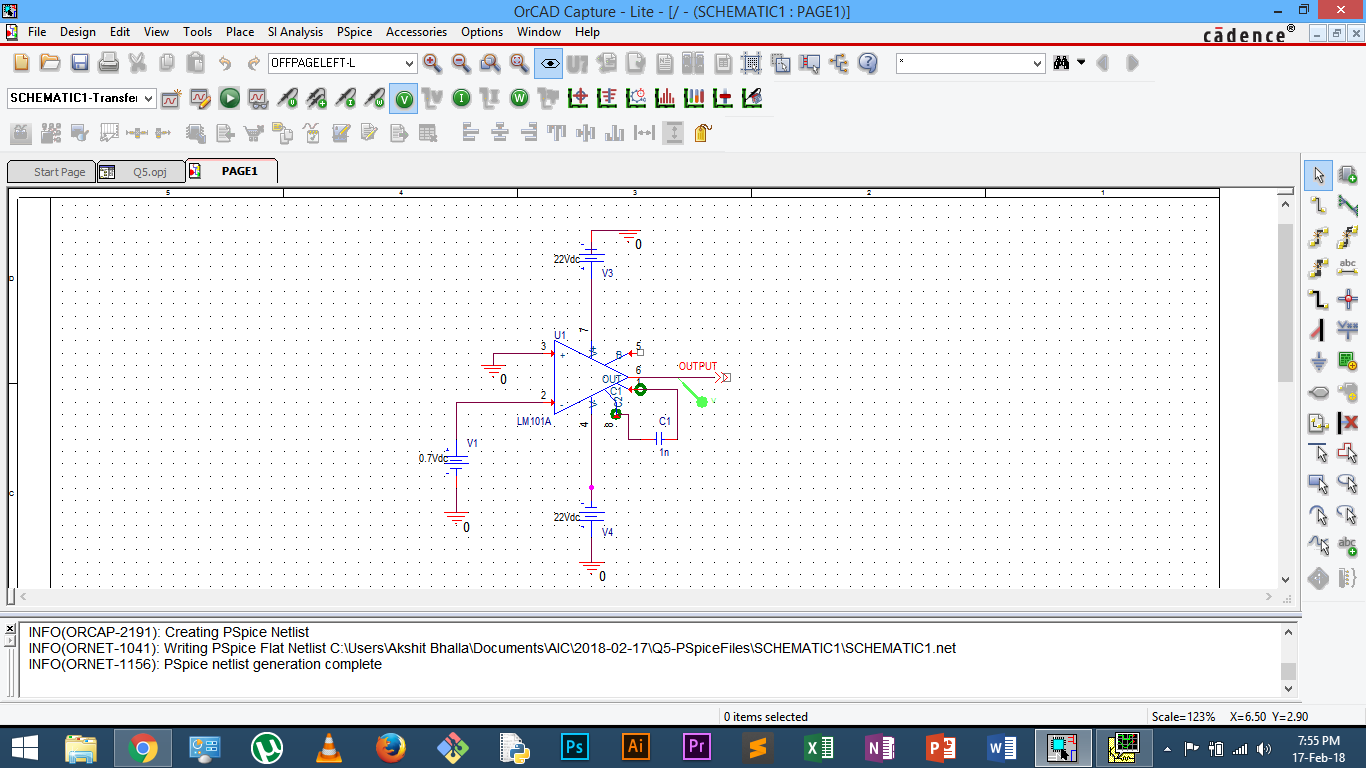
\includegraphics{Q5/origin}}  
	\centering
	\caption{Circuit Diagram}
	\label{fig:origin}
\end{figure}

\begin{figure}[H] 
	\centering
	\resizebox{12cm}{6cm}{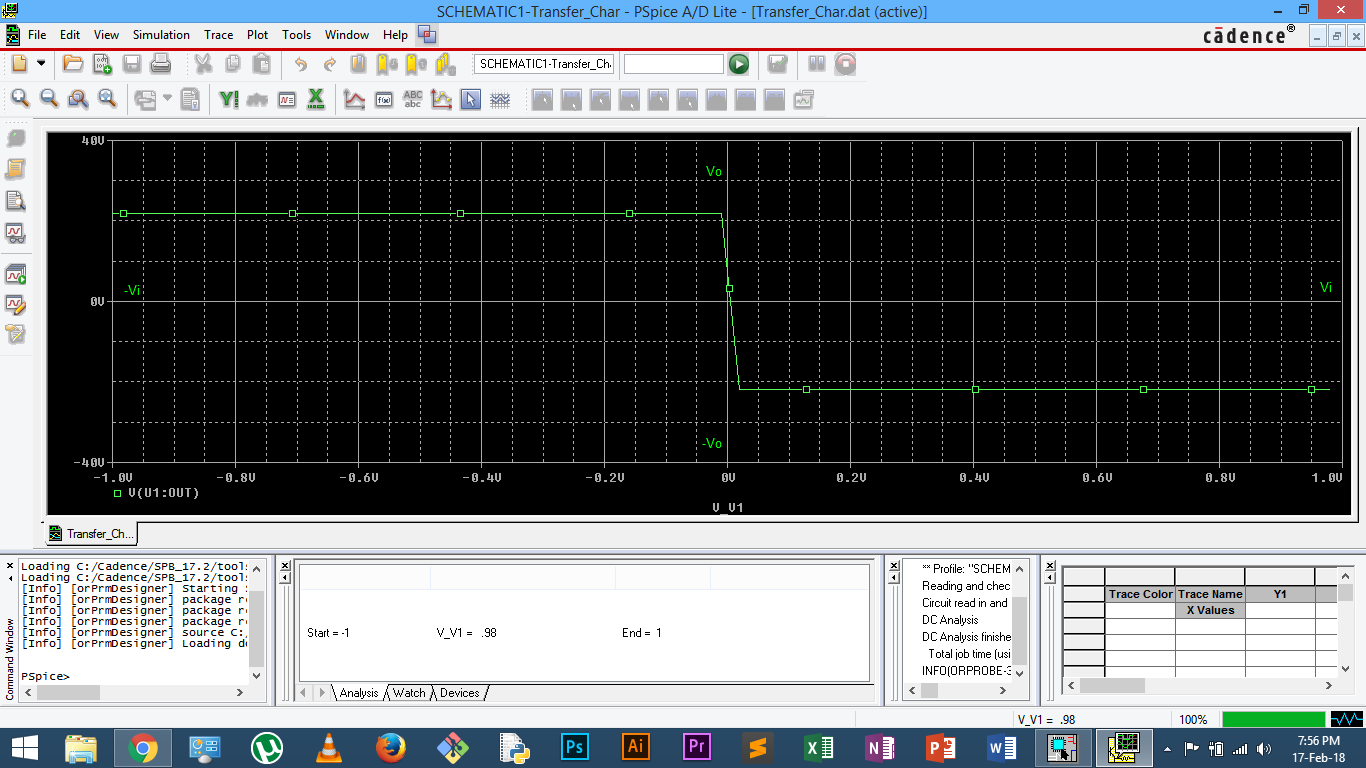
\includegraphics{Q5/origin1}}  
	\centering
	\caption{Transfer Characteristics}
	\label{fig:origin1}
\end{figure}

\pagebreak

\subsection*{Open Loop Configuration with Inverting and Non-Inverting Inputs - 1} \label{subsection:inv}

The circuit can be constructed as show in Figure \ref{fig:inv}. 

\begin{figure}[H] 
	\centering
	\resizebox{12cm}{6cm}{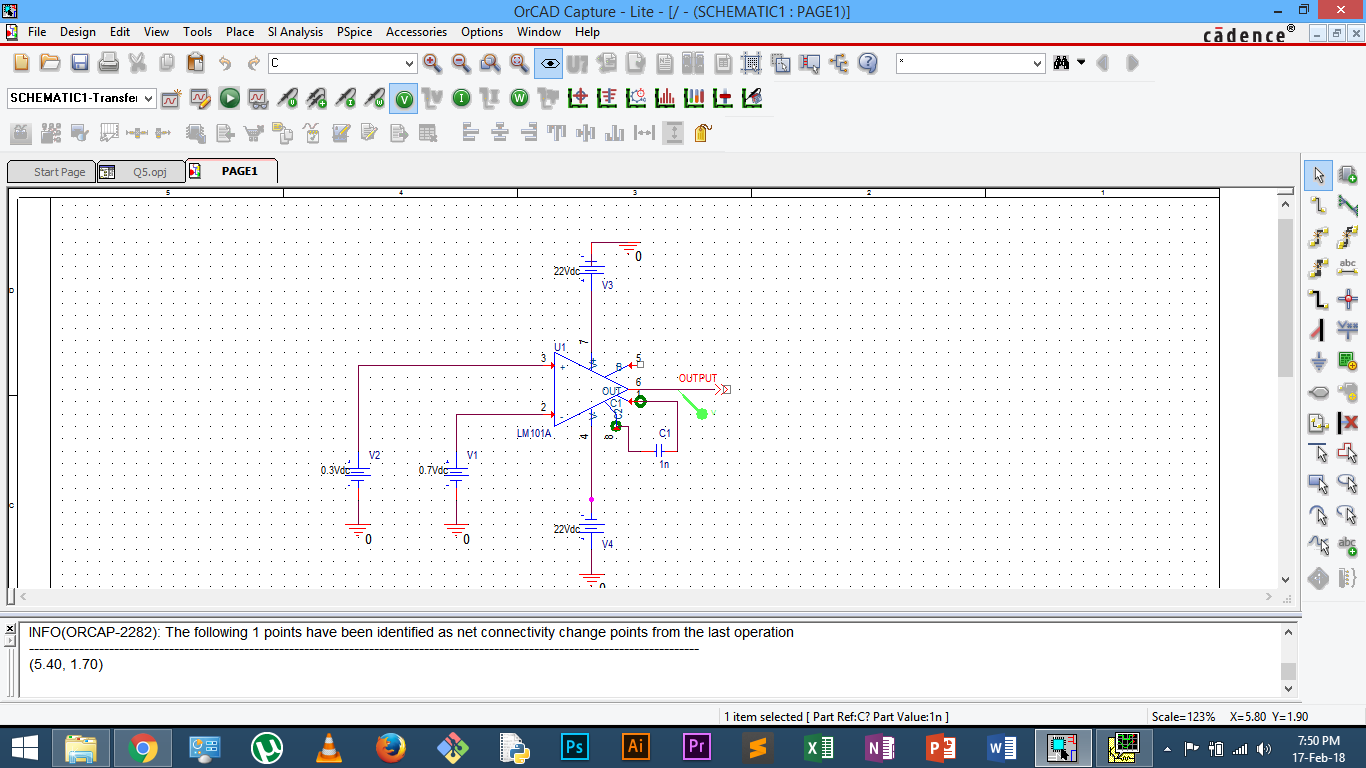
\includegraphics{Q5/inv}}  
	\centering
	\caption{Circuit Diagram}
	\label{fig:inv}
\end{figure}

\begin{figure}[H] 
	\centering
	\resizebox{12cm}{6cm}{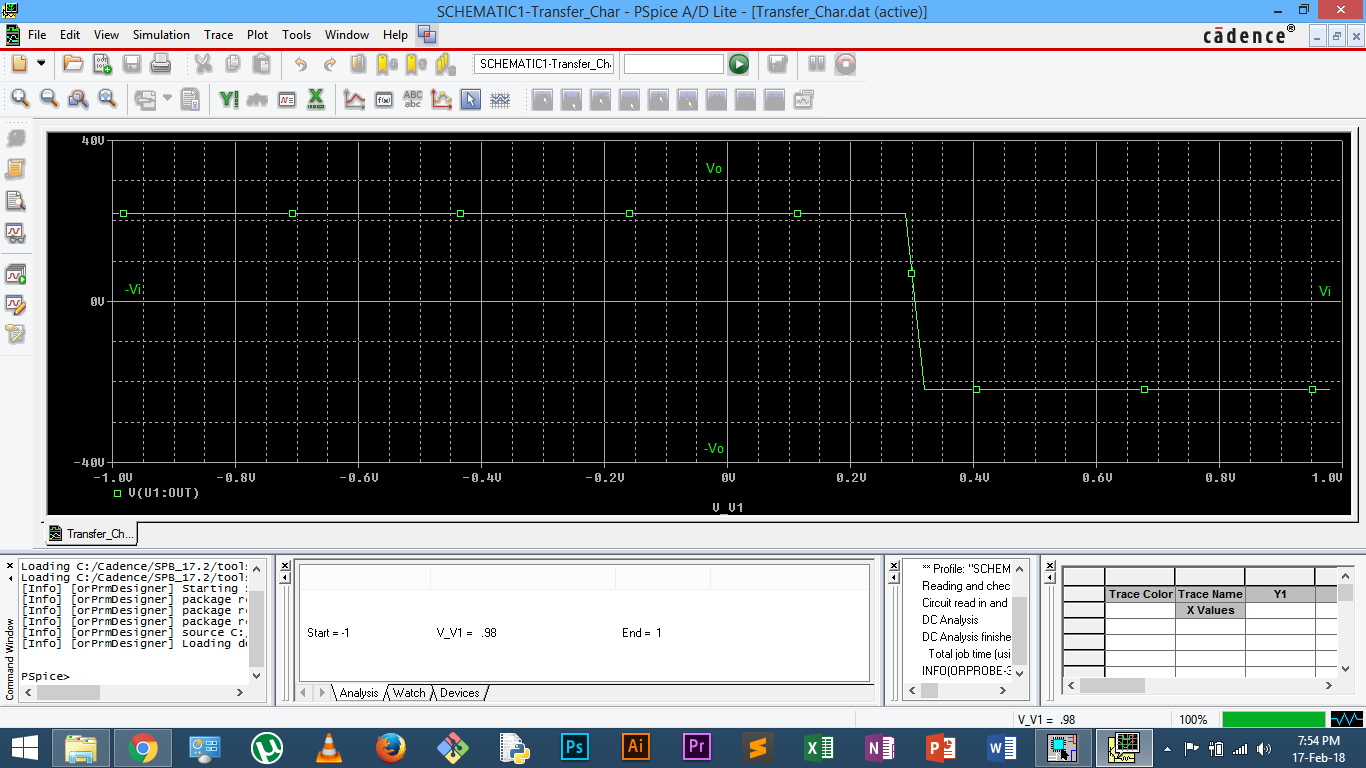
\includegraphics{Q5/inv1}}  
	\centering
	\caption{Transfer Characteristics}
	\label{fig:inv1}
\end{figure}

\pagebreak

\subsection*{Open Loop Configuration with Inverting and Non-Inverting Inputs - 2} \label{subsection:non-inv}

The circuit can be constructed as show in Figure \ref{fig:non-inv}. 

\begin{figure}[H] 
	\centering
	\resizebox{12cm}{6cm}{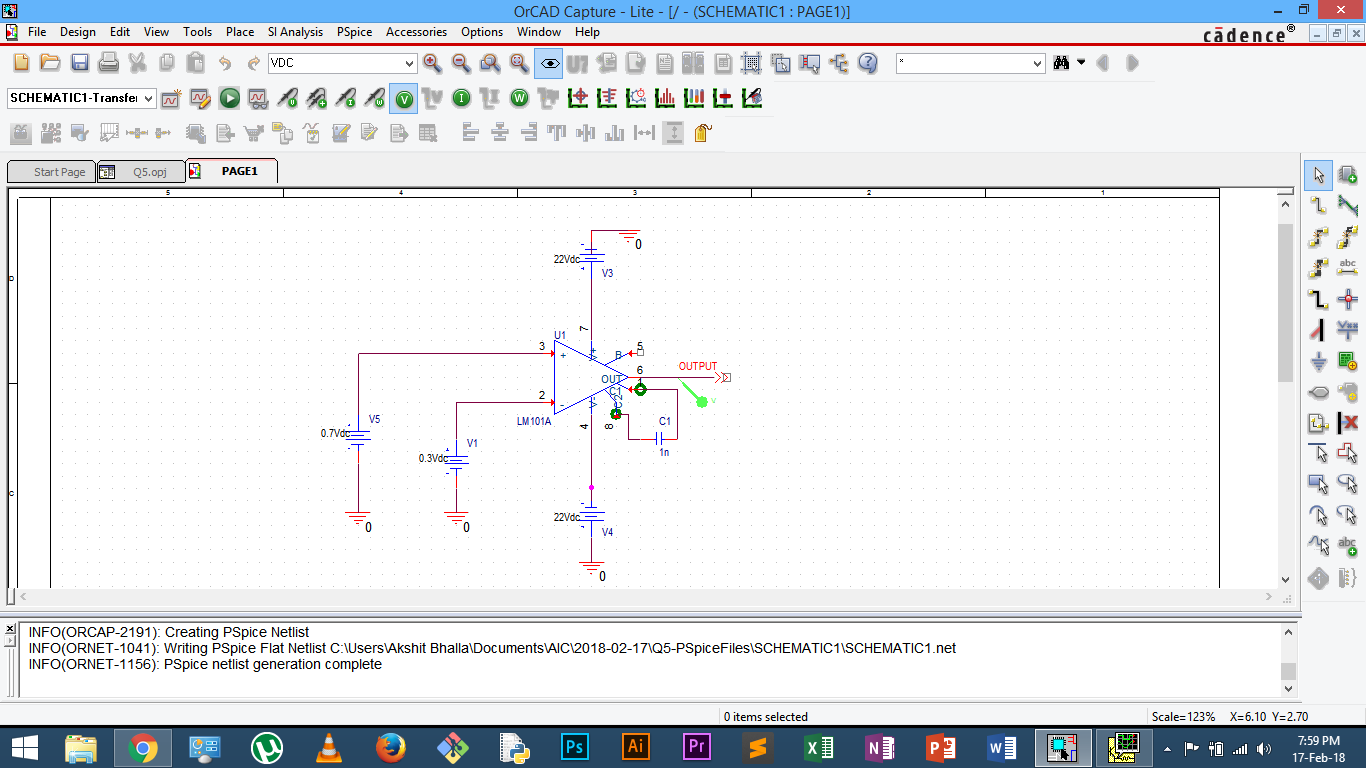
\includegraphics{Q5/non-inv}}  
	\centering
	\caption{Circuit Diagram}
	\label{fig:non-inv}
\end{figure}

\begin{figure}[H] 
	\centering
	\resizebox{12cm}{6cm}{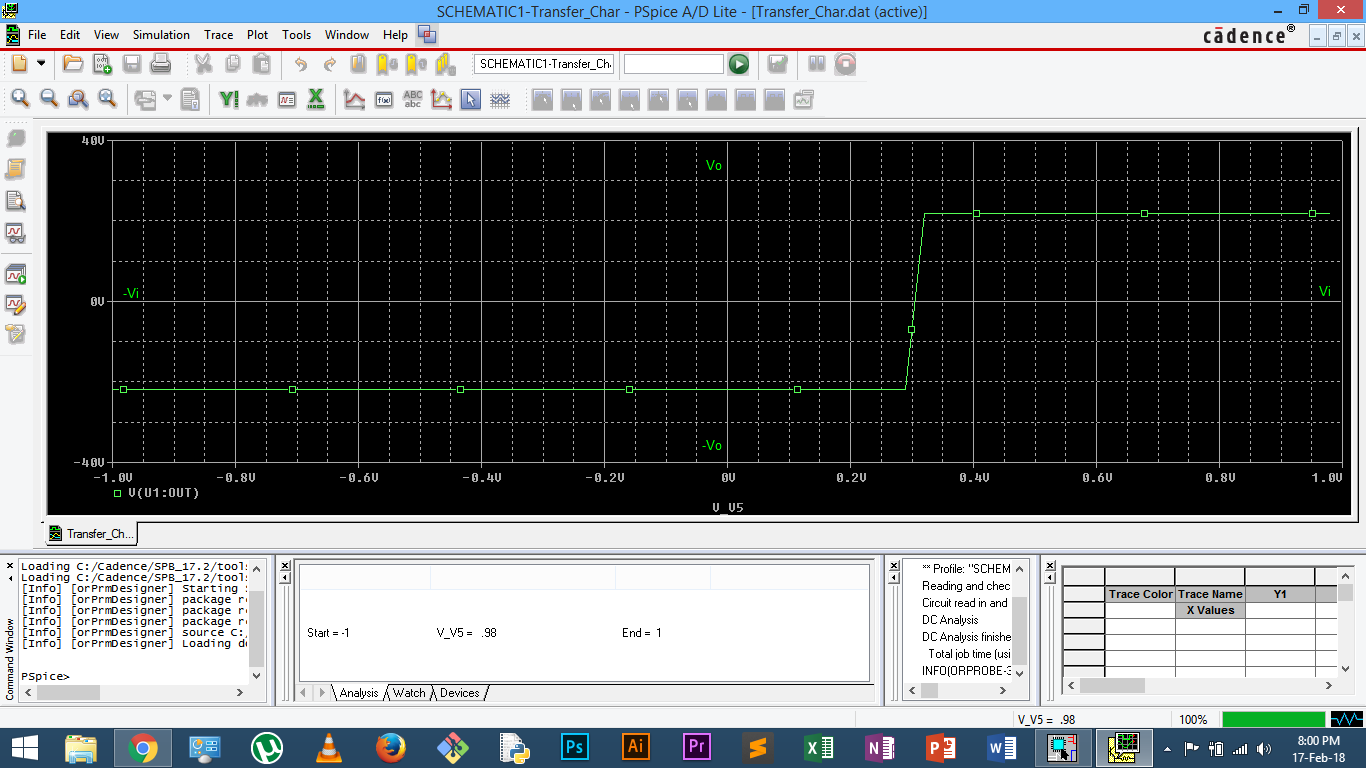
\includegraphics{Q5/non-inv1}}  
	\centering
	\caption{Transfer Characteristics}
	\label{fig:non-inv1}
\end{figure}
    
\end{homeworkProblem}

\pagebreak

\end{document}
